\section{Theorie}
\label{sec:Theorie}
Ein Laser (Light Amplification by
Stimulated Emission of Radiation)
besteht aus einem Resonator,
einer Pumpquelle und einem aktivem Lasermedium.
Damit ist es möglich, monochromatisches Licht mit einer
hohen Inensität und Kohärenz zu erzeugen.

\subsection{Absorption und Emission}
\label{subsec:absorption_und_emission}
Um die Funktionsweise eines Lasers
zu verstehen, ist es notwendig zunächst
die Wechselwirkung eines Niveau System
mit einem Strahlungsfeld $\rho(\nu)$ zu betrachten
Dazu zählen zum einen die Absorption eines Photon
und sowohl induzierte als auch spontane Emission eines Photon.
Zunachst soll der Fall
eines 2-Niveau Systems betrachtet
werden, wobei zwischen der Besetzungszahl $n_1$
der Atome im Grundzustand
und der Besetzungsdicht $n_2$
der Atome in angeregten
Zustand unterschieden wird.
Besitzt nun Beispielsweise ein
Photon die Energie des Übergangs
kann es von einem Atom im Grundzustand
absorbiert werden und das Atom geht in den
angeregten Zustand über. Atome im angeregten
Zustand können über spontane Emission
wieder in den Grundzustand zurückkehren
indem sie ein Photon mit der Energie
des Übergangs emittieren.
Dieser Übergang lässt ebenfalls
mit ein einfallendes
Photon hervorrufen.
Das so emittierte Photon besitzt gleiche
Energie, Phase und Ausbreitungsrichtung
wie das einfallende Photon,
üblicherweise ist dabei die Rede von
induzierte Emission.
Die Abbildung \ref{fig:ab_em} enthält die drei
zuvor beschriebenen möglichen Wechselwirkung.
\begin{figure}
  \centering
  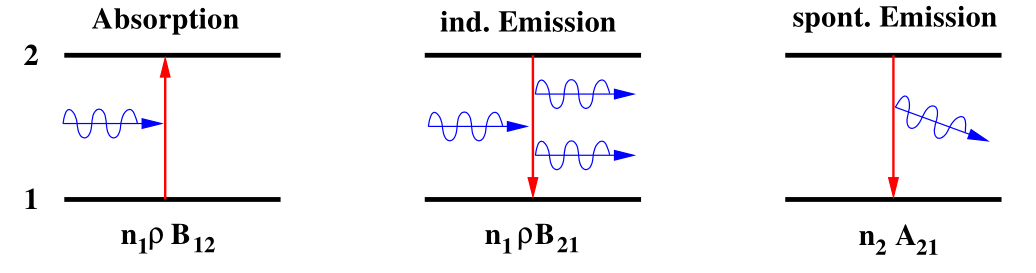
\includegraphics{figures/ab_und_emiss.PNG}
  \caption{Schematische Darstellung
  für die möglichen Wechselwirkung
   eines Strahlungsfeld
  mit einem 2-Niveau System. \cite{sample}}
  \label{fig:ab_em}
\end{figure}

Die Anzahl der so
pro Volumeneinheit und pro Sekunde
absorbiert/emittierten Photonen $\dot{N}$,
ergeben sich mit den Einsteinkoeffizienten $A_21$, $B_21$ und $B_12$
und der Energiedichte $\rho$ des Strahlungsfeldes zu
\begin{align}
& \text{Absorption}   &\dot{N}_A   &= n_1 \rho(\nu)B_{12},\\
& \text{induzierte Emission}   &\dot{N}_{IE}&= n_2 \rho(\nu)B_{21},\\
& \text{spontane Emission}   &\dot{N}_E   &= n_2 \rho(\nu) A_{21}.
\end{align}

Die Einsteinkoeffizienten $A_21$, $B_21$ und $B_12$
geben ein Maß für die Übergangswahrscheinlichkeiten an.
Für eine verlustfreie Vorgang
$(n_1+n_2=const.)$ ändern sich die Bestzungszahlen
gleichermaßen und es ergeben sich folgende
Ratengleichungen für die Besetzungszahlen
\begin{align}
\frac{\symup{d} n_1}{\symup{d} t} &=-n_1 B_{21}\rho + N_2 B_{21} \rho + n_2 A_{21}\\
\frac{\symup{d} n_2}{\symup{d} t} &=+N_1 B_{12}\rho - n_2 B_{21} \rho - n_2 A_{21}.
\end{align}
Damit eine dauerhafte Verstärkung
und Kohärenz des Strahlungsfeld gegeben ist,
muss mehr induzierte als spontane Emission
statt finden. Um dies zu
erreichen wird eine Besetzungsinversion
zwischen Angeregtem- und Grundzustand
erzeugt.
Da im thermischen Gleichgewicht
die Besetzungszahlen sich nach der
Maxwell-Boltzmann-Verteilung
richtet, ist der Grundzustand höher
besetzt als der angeregte Zustand.
Um eine Besetzungsinversion zu erreichen
muss somit dem System kontinuierlich
Enerige Beispielsweise durch
Elekronenstöße oder
optische Anregung zugeführt werden.
Dieser Vorgang wird auch Pumpen genannt.



\subsection{Konzeptioneller Aufbau des Lasers}
\label{subsec:konzeptioneller_aufbau}


\subsection{Lasermoden}
\label{subsec:lasermoden}
